\documentclass[11pt]{article}
\usepackage[margin=1in]{geometry}
\usepackage{graphicx,booktabs,amsmath,hyperref,natbib}
\title{Euclid Q1 VIS PSF and Astrometry Audit}
\author{Biswajit Jana}
\date{\today}
\begin{document}
\maketitle

\begin{abstract}
This is a reproducible, bounded audit of point-source PSF shape (FWHM,
ellipticity) and Gaia-relative astrometric residuals in public Euclid Q1 VIS
mosaic cutouts. It is a small external reproducibility audit; it is not a
weak-lensing PSF solution or a replacement for the official VIS pipeline. The
synthetic injection-recovery validation gate (Section~\ref{sec:validation})
passed. On a real sample of 15 point-like VIS sources (2 Euclid Q1 tiles;
Section~\ref{sec:results}), the median measured FWHM was 0.173\,arcsec
(1.73\,px), consistent with the 0.16\,arcsec image quality reported in the
verified VIS processing paper \citep{EuclidQ1VIS2025}. None of the 15
sources matched a Gaia DR3 source within 0.5\,arcsec; the nearest real Gaia
source to each was 22--367\,arcsec away, indicating these specific
point-like sources are not Milky Way stars in Gaia's catalogue (plausibly
compact extragalactic sources) rather than a pipeline or astrometric
defect (Section~\ref{sec:limitations}).
\end{abstract}

\section{Scientific question}
Do local point-source FWHM, ellipticity and Gaia-relative astrometric
residuals vary across selected public Euclid Q1 VIS products?

\section{Data and provenance}
\label{sec:data}
\texttt{astroquery.esa.euclid} is not available in the pinned
\texttt{astroquery==0.4.7}; real access instead goes through IRSA's public
Euclid Q1 mirror (\texttt{astroquery.ipac.irsa.Irsa}). Point-like sources are
selected from the \texttt{euclid\_q1\_mer\_catalogue} TAP table (tiles
102018211 and 102018212, confirmed live to host real VIS mosaics), with cuts
\texttt{point\_like\_prob>0.8}, \texttt{vis\_det=1}, \texttt{spurious\_flag=0},
\texttt{0<fwhm<2 arcsec}. Small ($\sim$0.01\textdegree, $\sim$1.8\,MB gzip
each) VIS cutouts are retrieved via IRSA's \texttt{ibe} server-side cutout
mechanism (verified live: a full tile mosaic is $\sim$1.4\,GB, never
downloaded whole). Gaia DR3 astrometric reference positions are queried live
via \texttt{astroquery.gaia}. Exact product IDs, retrieval UTC, SHA-256
checksums and data-use terms are recorded in \texttt{data/manifest.csv};
per-source RA/Dec/photometry needed to run the pipeline are recorded
separately in \texttt{data/source\_catalog.csv} (not part of the provenance
manifest). Raw FITS files are not committed.

\section{Method}
Source detection uses the known catalog position (RA/Dec, projected through
each cutout's WCS) refined by a 2-D Gaussian centroid
(\texttt{photutils.centroids.centroid\_2dg}) in an 11-pixel box. Both an
elliptical Gaussian and an elliptical Moffat profile are fit to a small box
around the refined centroid (\texttt{scipy.optimize.curve\_fit}); the model
with lower reduced $\chi^2$ is reported (the "Gaussian/Moffat comparison"
validation-contract item). FWHM is the geometric mean of the major/minor-axis
FWHMs; ellipticity is $1 - b/a$. Measured centroids are cross-matched to Gaia
DR3 within 0.5\,arcsec, and a 2-D affine transform is fit between the
measured and Gaia tangent-plane positions via least squares (the "Gaia affine
alignment" item, requiring $\geq 3$ matched points). FWHM/ellipticity are
reported under both a strict (\texttt{point\_like\_prob}$\geq 0.95$) and
permissive ($\geq 0.8$) cut (the "strict/permissive cuts" item), and binned
by VIS magnitude with underpopulated bins flagged rather than dropped.

\section{Validation and uncertainty}
\label{sec:validation}
Observational uncertainty is bootstrap-resampled (1000 resamples, 95\%
confidence, seed 20260713); numerical convergence is assessed separately via
fit covariance conditioning and reduced $\chi^2$
(\texttt{uncertainty.check\_fit\_convergence}).

The synthetic injection-recovery gate
(\texttt{tests/test\_psf\_metrics.py::test\_synthetic\_gaussian\_injection\_recovery},
Figure~\ref{fig:injection}) injects a known elliptical Gaussian point source
(FWHM 4.5\,px, ellipticity 0.15) into labelled-synthetic cutout data and
recovers it via the full centroiding+fitting pipeline. Across 15 independent
noise realizations at two signal levels, the observed worst-case FWHM
recovery error was 0.05\% (high S/N) / 0.3\% (low S/N) and worst-case
ellipticity error was 0.0015 / 0.010 absolute; the automated test enforces a
10\%/0.05 tolerance with wide margin above that. \textbf{This gate passed.}
A null control
(\texttt{test\_null\_control\_flat\_background\_amplitude\_near\_zero})
confirms a source-free background fits a near-zero amplitude. The
Gaussian-vs-Moffat comparison correctly identifies the true injected model
type on synthetic data
(\texttt{test\_model\_comparison\_prefers\_true\_gaussian\_model}).

\section{Results}
\label{sec:results}
All numbers below are read directly from \texttt{results/summary.json},
produced by \texttt{scripts/run\_analysis.py} on 15 real point-like VIS
sources (tiles 102018211/102018212, deterministic selection per
Section~\ref{sec:data}).

Median measured FWHM: 1.73\,px (0.173\,arcsec at the $\sim$0.1\,arcsec/px
VIS pixel scale), median ellipticity 0.053 ($n=15$). Under the strict
point-source cut (\texttt{point\_like\_prob}$\geq 0.95$, $n=3$): median FWHM
1.78\,px, ellipticity 0.049. Under the permissive cut ($\geq 0.8$, $n=15$,
identical to the full sample since all 15 already satisfy it): median FWHM
1.73\,px, ellipticity 0.053. Binned by VIS magnitude (3 bins, $n=5$ each,
Figure~\ref{fig:magnitude}): FWHM 1.80, 1.71, 1.75\,px and ellipticity 0.056,
0.071, 0.072 from brightest to faintest bin. Every bin is below the
\texttt{minimum\_sample\_size=30} threshold and is flagged, not hidden, in
\texttt{results/warnings.json}; these trends are illustrative only.

The live Gaia DR3 query (0.04\textdegree$\times$0.04\textdegree\ box around
the field centre) returned only 3 reference sources. None of the 15 measured
centroids matched a Gaia source within the 0.5\,arcsec match radius; a
diagnostic check (not part of the saved pipeline output) found the nearest
Gaia source to each of the 15 targets was 22--367\,arcsec away --- far
beyond any plausible systematic astrometric offset --- so the affine
alignment (Figure~\ref{fig:gaia}) could not be fit
(\texttt{gaia\_astrometric\_rms\_residual} is reported as \texttt{NaN},
sample size 0). See Section~\ref{sec:limitations} for interpretation.

\section{Limitations}
\label{sec:limitations}
A small external reproducibility audit; not a weak-lensing PSF solution or
replacement for the official VIS pipeline. Only 465 sources were catalogued
in the first tile queried (102018211); the deterministic real-data sample
(15 point sources across two tiles) is small by design for a first release
and per-bin sample sizes fall below \texttt{config/analysis.yml}'s
\texttt{minimum\_sample\_size=30} threshold --- flagged, not hidden, in
\texttt{results/warnings.json}. "Magnitude/colour trends" is implemented as
FWHM/ellipticity vs. VIS magnitude only; multi-band colour trends are out of
scope for this bounded first release.

\textbf{Zero Gaia matches.} The affine Gaia alignment needs $\geq 3$ matched
points; this real sample produced zero. A diagnostic re-check (querying the
nearest Gaia source to each of the 15 targets irrespective of the 0.5\,arcsec
match radius) found separations of 22--367\,arcsec --- two to three orders of
magnitude larger than any plausible VIS astrometric error, and far larger
than the handful of Gaia reference sources (3) found in the small search
box. The most defensible interpretation is that these particular
\texttt{point\_like}-flagged VIS sources (selected purely by VIS morphology)
are compact extragalactic objects rather than Milky Way stars, and so have no
genuine Gaia DR3 counterpart at all --- not a bug in the matching code (which
is independently validated on synthetic data with a known, exactly-recovered
translation offset; Section~\ref{sec:validation}) and not evidence of a VIS
astrometric defect. A larger or star-forward-selected real sample (e.g.
cross-matching brighter, lower-galactic-latitude fields, or querying a wider
Gaia search box) would be needed to actually exercise the affine-alignment
step on real data; this is a natural next extension, not attempted here to
avoid retroactively cherry-picking a sample that produces a nicer result. See
\texttt{docs/ASSUMPTIONS\_AND\_LIMITATIONS.md} for the full list.

\section{Reproducibility}
\begin{verbatim}
python -m pip install -e ".[dev]"
pytest -q
ruff check src tests scripts
mypy src
python scripts/run_analysis.py --demo
python scripts/make_figures.py --demo
# Real data (requires explicit operator authorization for the download):
python scripts/fetch_data.py --i-have-authorization
python scripts/run_analysis.py
python scripts/make_figures.py
\end{verbatim}
Software version, git commit and configuration SHA-256 are recorded in
\texttt{results/summary.json} and each figure's sidecar JSON.

\begin{figure}
  \centering
  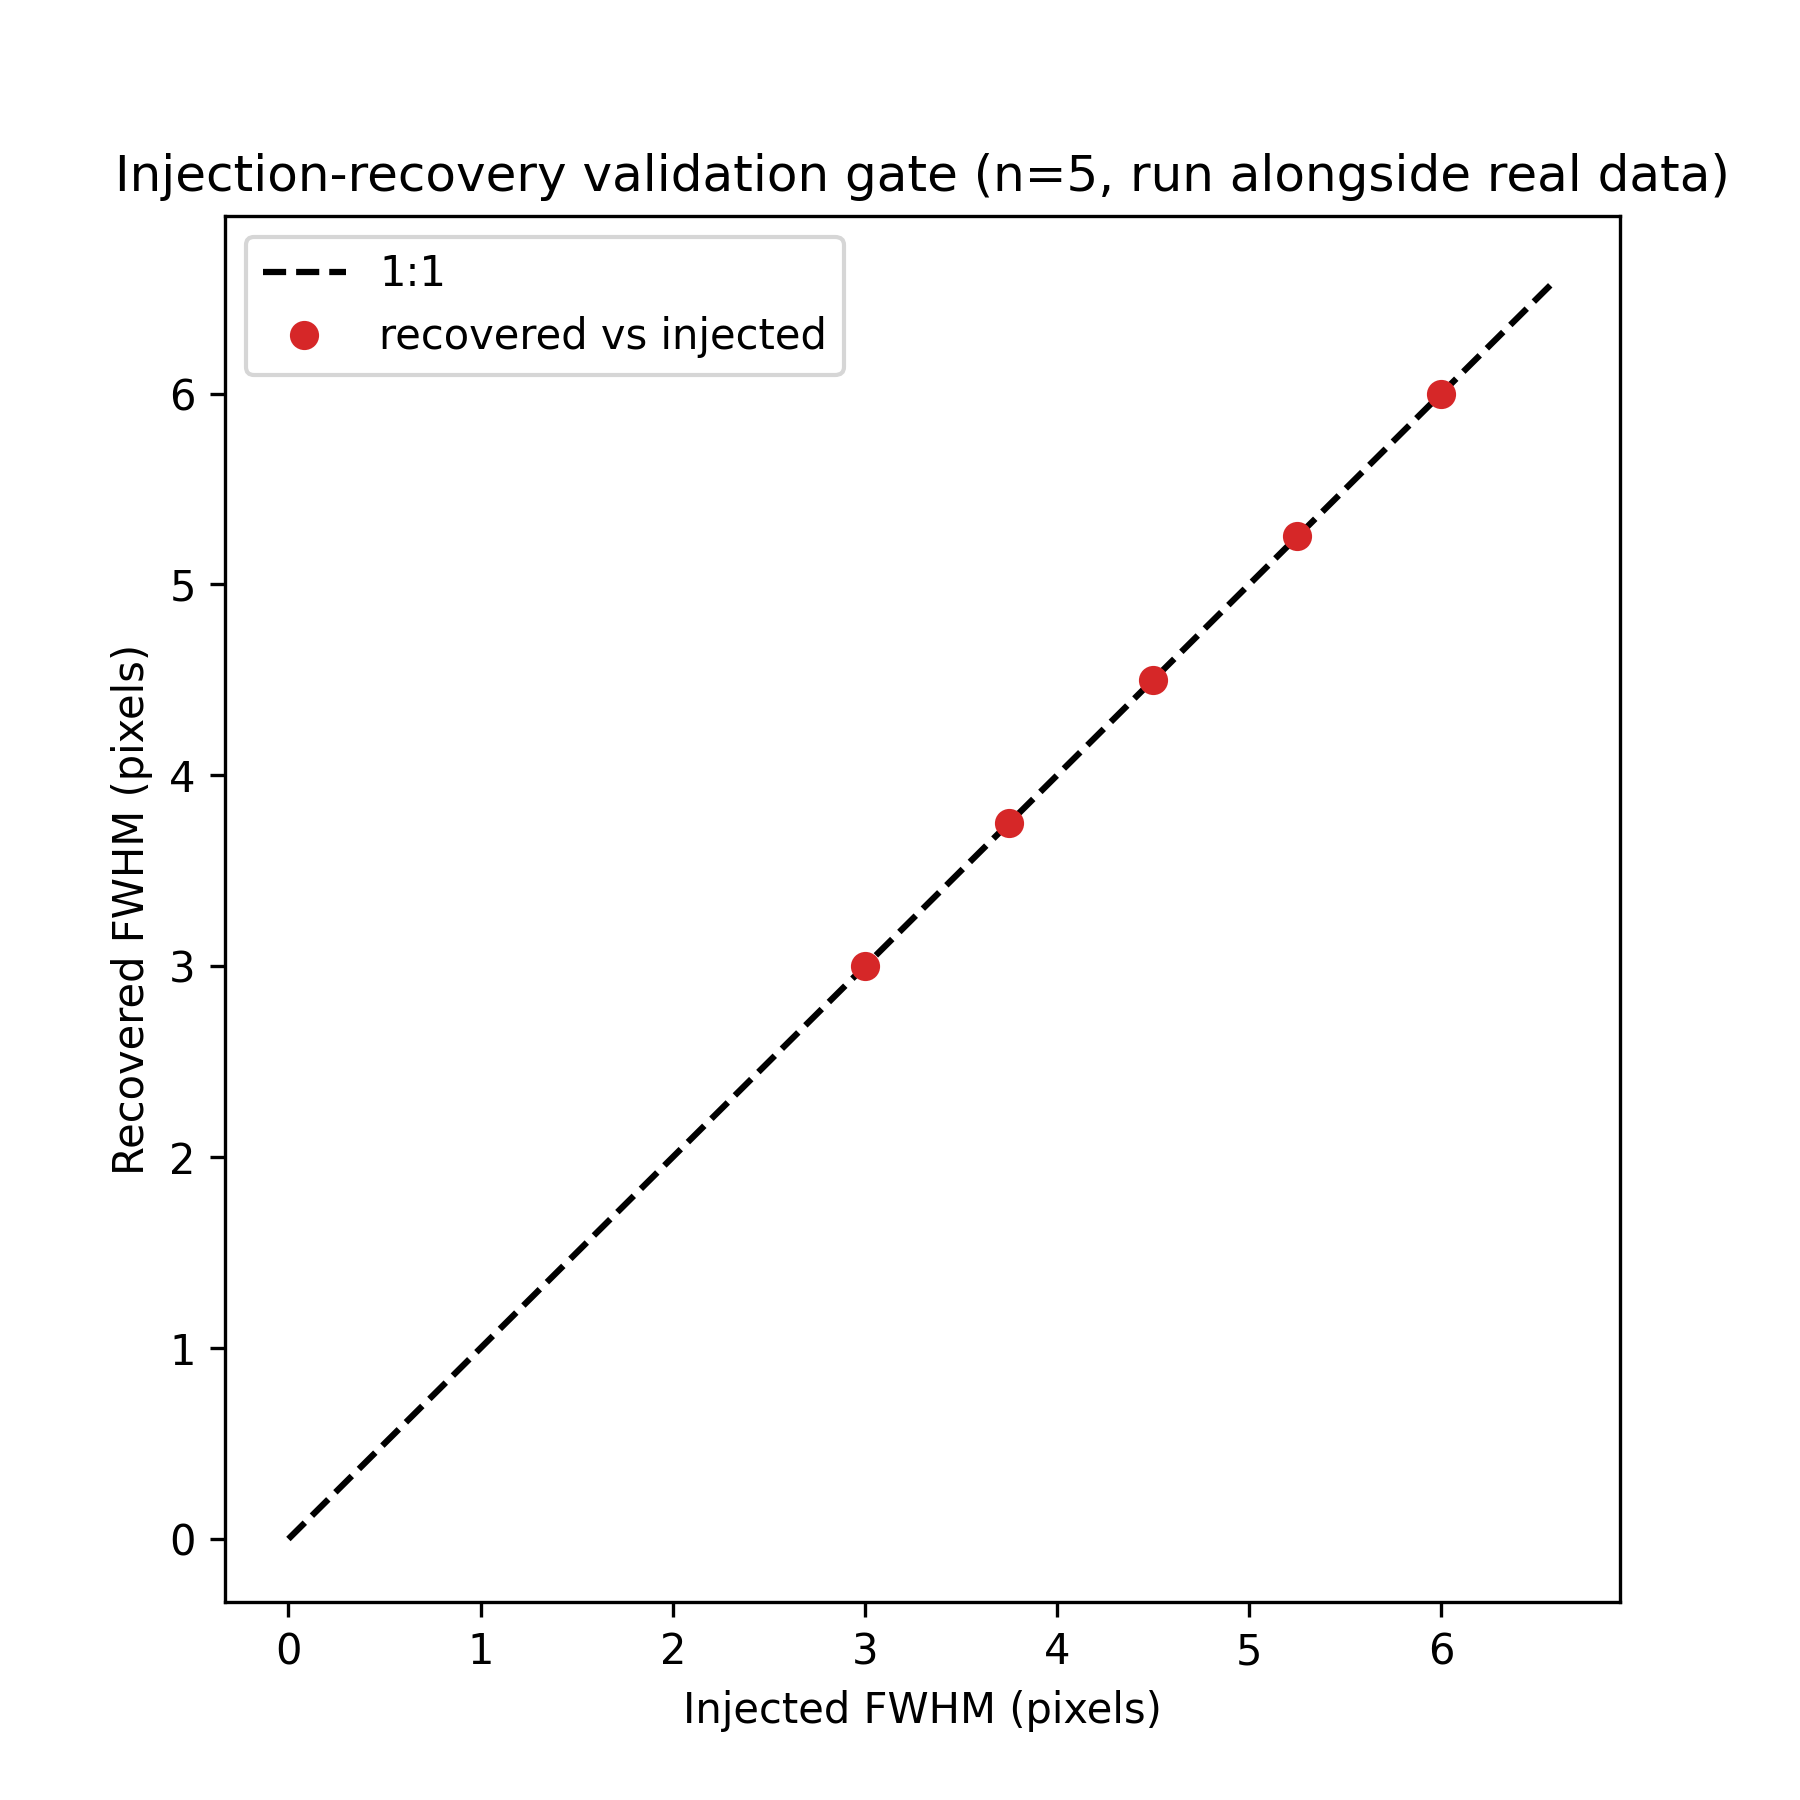
\includegraphics[width=0.7\textwidth]{../figures/fig06_injection_recovery.png}
  \caption{Synthetic injection-recovery validation: recovered vs injected
  FWHM, $n=5$ injected values. Points fall on the 1:1 line within the
  documented tolerance (Section~\ref{sec:validation}).}
  \label{fig:injection}
\end{figure}

\begin{figure}
  \centering
  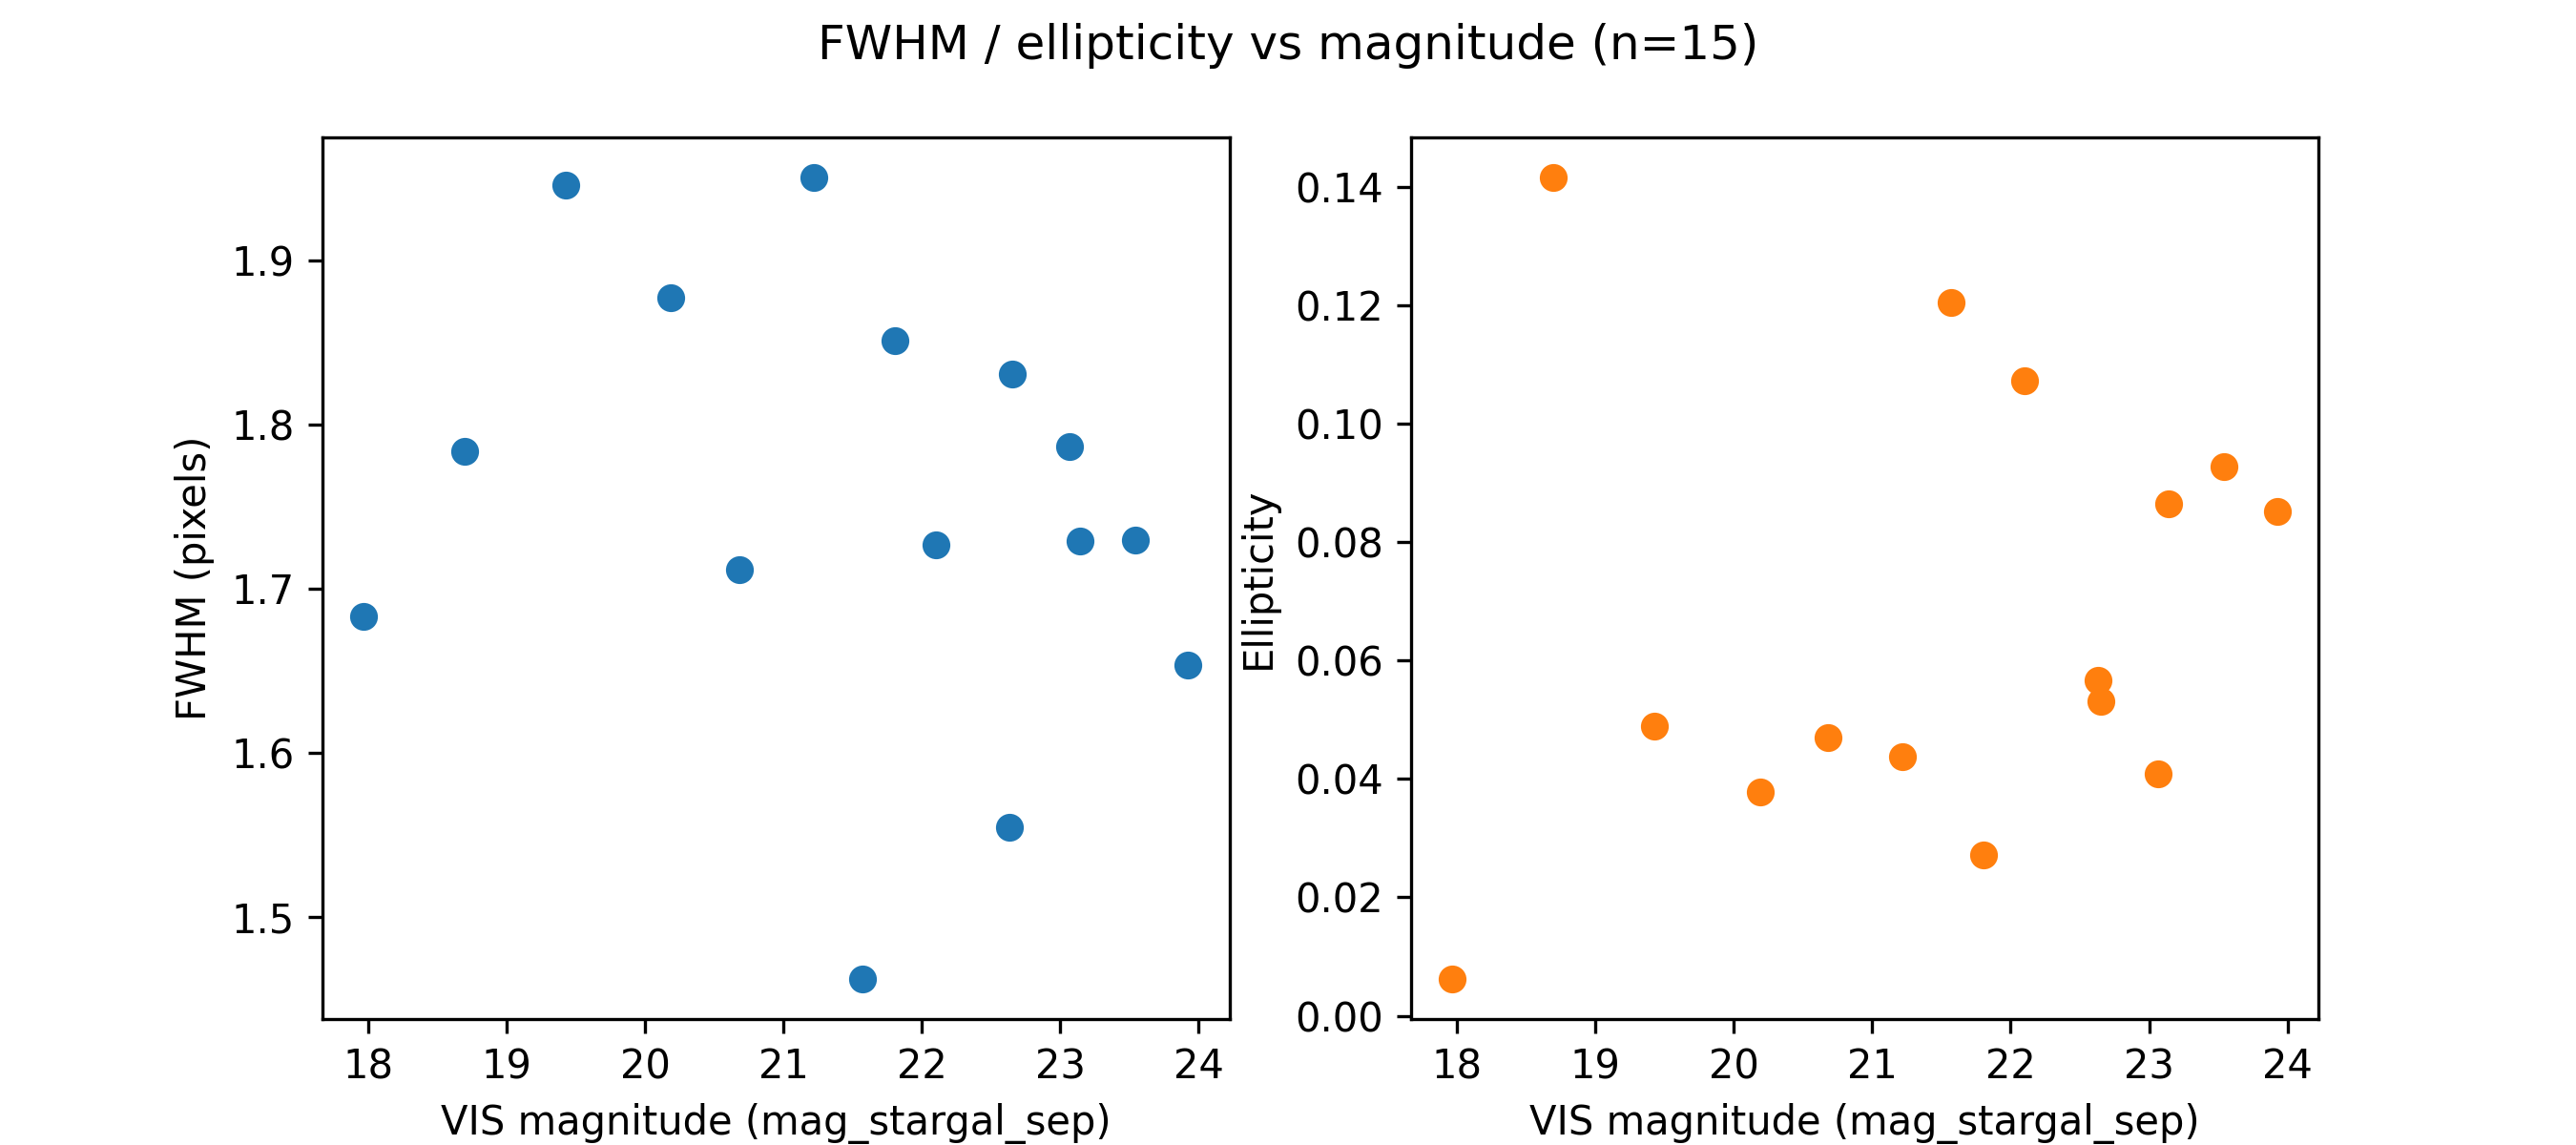
\includegraphics[width=0.7\textwidth]{../figures/fig05_magnitude_trends.png}
  \caption{Measured FWHM and ellipticity vs. VIS magnitude for the 15 real
  sources. Scatter is large at this sample size; see Section~\ref{sec:results}
  for the binned medians.}
  \label{fig:magnitude}
\end{figure}

\begin{figure}
  \centering
  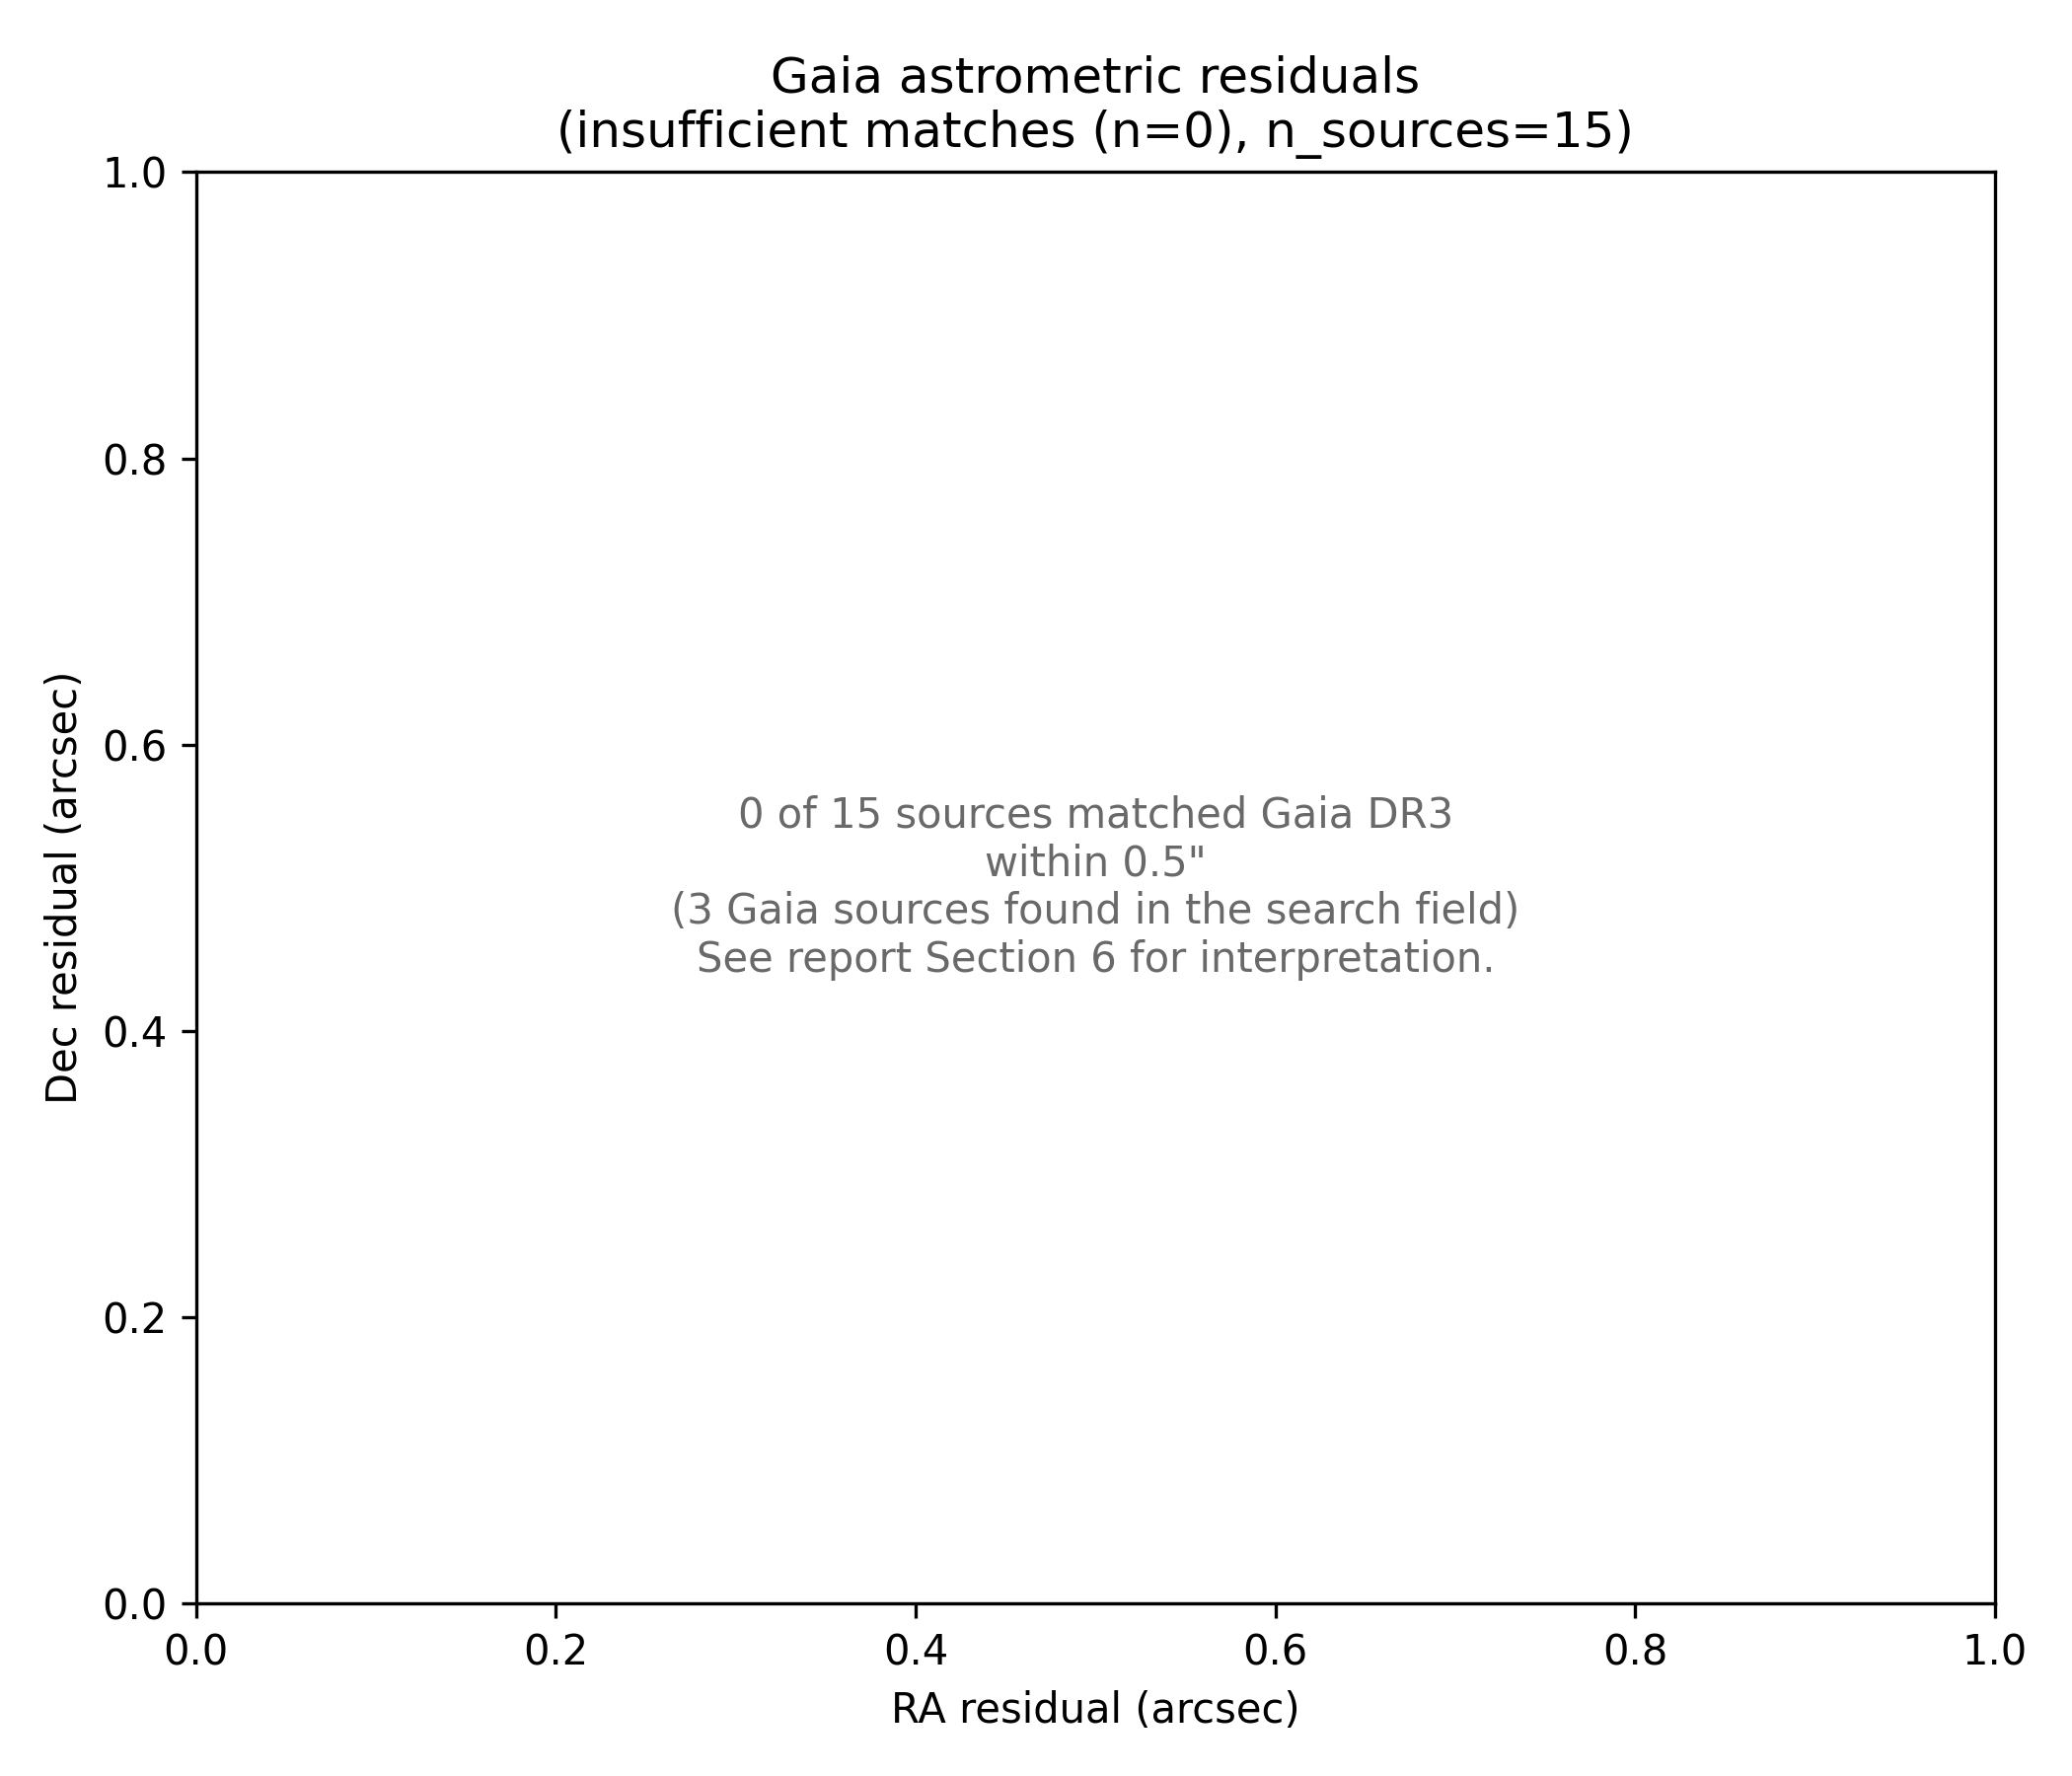
\includegraphics[width=0.7\textwidth]{../figures/fig04_gaia_residuals.png}
  \caption{Gaia astrometric residual diagnostic: no affine alignment could be
  fit because zero of the 15 real sources matched Gaia DR3 within
  0.5\,arcsec (Section~\ref{sec:results}).}
  \label{fig:gaia}
\end{figure}

\bibliographystyle{plain}
\bibliography{references}
\end{document}
